\documentclass{beamer}
\usetheme{Antibes} 
\usepackage{textcomp}
\begin{document}
	\title{Mashbot}
	\author{Andrew Gall, Vito Salerno, Josiah Kiehl, G. Nicholas D'Andrea, and Cody Ray}
	\date{\today}

	\frame{\titlepage}
	
	\section{Rationale}
		\frame{
			\frametitle{Social Media is Complicated}
			\begin{itemize}
				\item Lots of services already
				\item Every site/API is different
				\item Always new services coming out
			\end{itemize}
		}
		\frame{
			\frametitle{Small Business Owners Are Busy}
			\begin{itemize}
				\item Many are one man or small operations
				\item They are busy creating their product
				\item No time to worry about their web presence
				\item No time to learn
			\end{itemize}
		
		}
		\frame{
			\frametitle{Let's Help Them Maintain Their Online Presence}
			\begin{itemize}
				\item Offer an intuitive interface that can be learned quickly
				\item Offer a wide range of services to give them maximum exposure
				\item Allow them to plan their marketing outside of the busy season
			\end{itemize}
		
		}
		\frame{
			\frametitle{Solving the Larger Problem}
			\begin{itemize}
				\item Why should we just code up a specific solution to just this 
					problem?
				\item Connecting to lots of services
				\item Make a foundation which is a concrete stepping block towards 
					solving the problem of interacting with the social media explosion
		
			\end{itemize}
		
		}

	\section{Architecture}
		\frame{
			\frametitle{Overview}
		
                  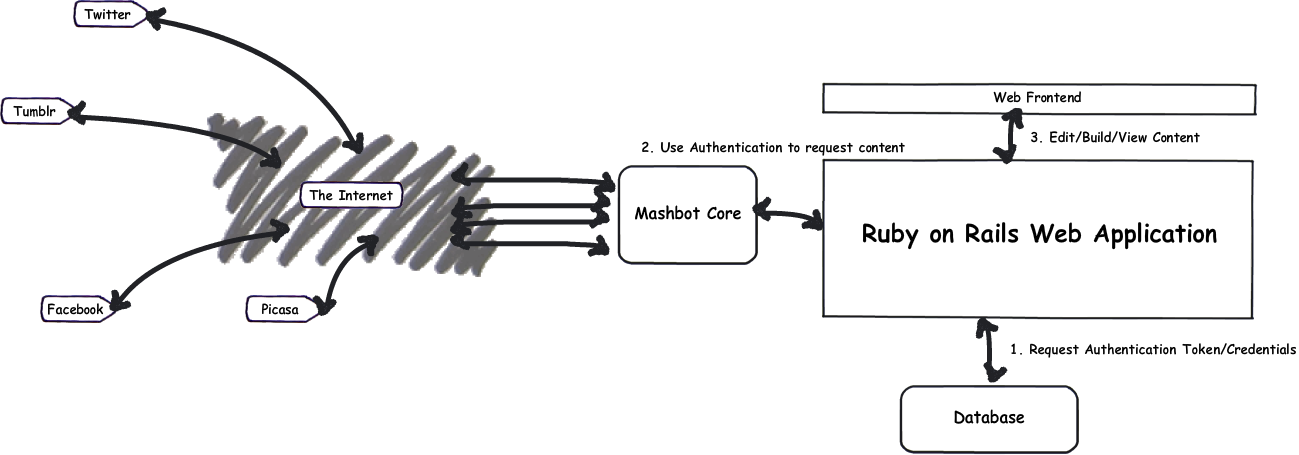
\includegraphics[width=\textwidth]{../mockups/dataflow.png}
		}
		\frame{
			\frametitle{Overview}
                        \begin{itemize}
                        \item Write once, post anywhere
                        \item Include new services via plugins
                        \item Application platform
                        \end{itemize}
		}
		\frame{
			\frametitle{Write once, post anywhere}
                        \begin{itemize}
                          \item Stateless Publishing and Aggregation Platform
                          \item Send to as few or as many services as the user has supplied credentials for
                          \item Asynchronous Worker Queue
                        \end{itemize}
		}
		\frame{
			\frametitle{Include new services via plugins}
                        \begin{itemize}
                          \item Will ship with several supported services
                          \item As new services are released, developers can write plugins for the Publishing and Aggregation Platform as well as the Campaign Manager
                          \item Mashbot is content type agnostic!
                        \end{itemize}
		}
		\frame{
			\frametitle{Application Platform}
                        \begin{itemize}
                          \item Publishing and Aggregation Platform does not know anything about the Campaign Manager.
                          \item Handle requests, return data.  Not coupled with any application.
                          \item Open Source
                        \end{itemize}
		
		}

	\section{Publishing and Aggregation Platform}
		\frame{
			\frametitle{Not Just An Application}
			\begin{itemize}
				\item Campaign manager is just an example of what can build on our 
					platform
				\item Building an underlying general service for interacting with social 
					media
			\end{itemize}
		}
		\frame{
			\frametitle{What It Offers?}
			\begin{itemize}
				\item Unified access to any service we support
				\item Flexibility to easily add new services quickly
				\item Ability to support new types of content easily
				\item Easy to configure
			\end{itemize}
		}
		
		\frame{
			\frametitle{How We Are Building It}
			\begin{itemize}
				\item Language: Java
				\item Platform: Apache CXF and Spring
				\item Type of Service: REST
			\end{itemize}
		}

		\frame{
			\frametitle{Internal Architecture}
			\begin{itemize}
				\item Emphasize on decoupling for easy testing
				\item Handler Chain
				\item Plugins are configured at run time
			\end{itemize}
		}

	\section{Visual Design}
		\frame{
                  \frametitle{}
		
                  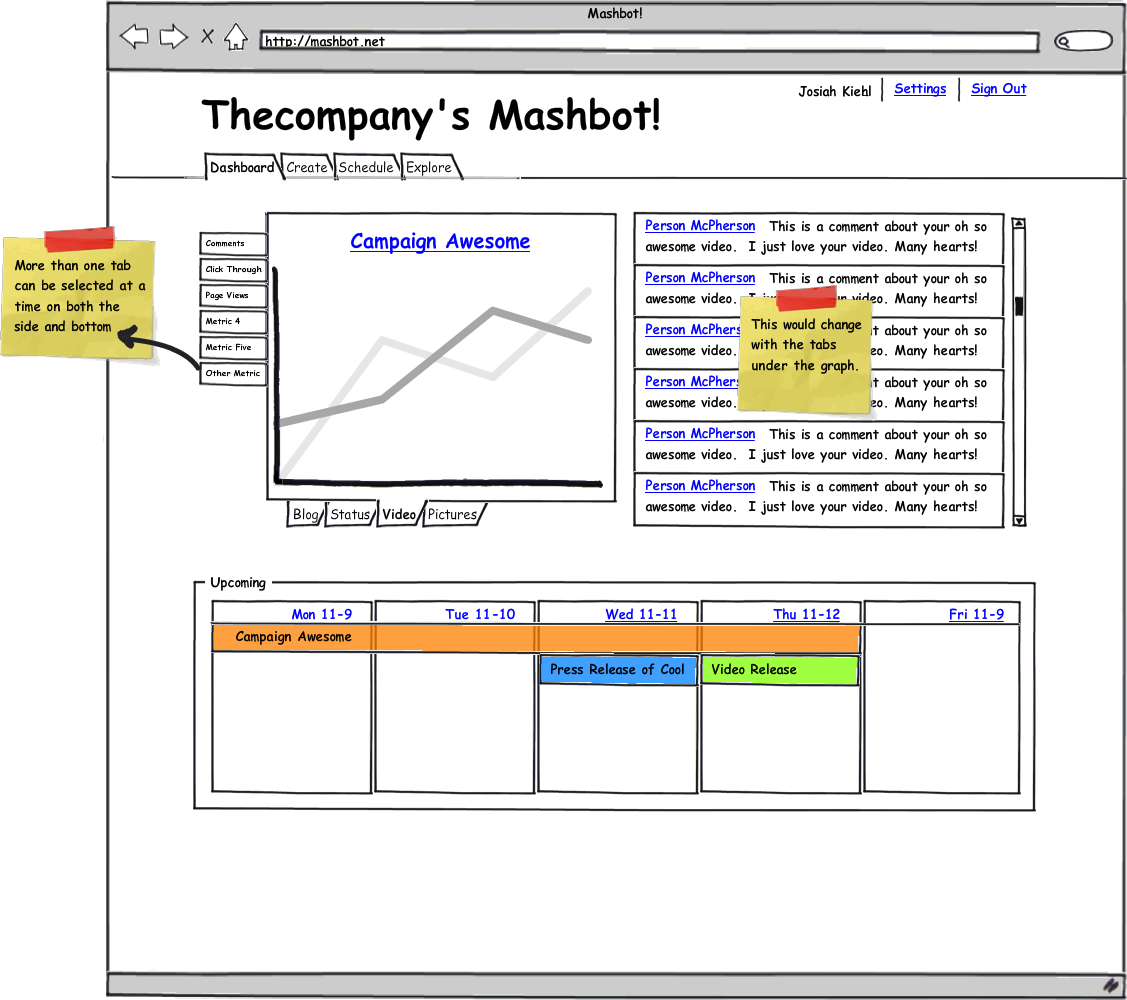
\includegraphics[width=\textwidth]{../mockups/dashboard.png}
		}
		\frame{
			\frametitle{}

                  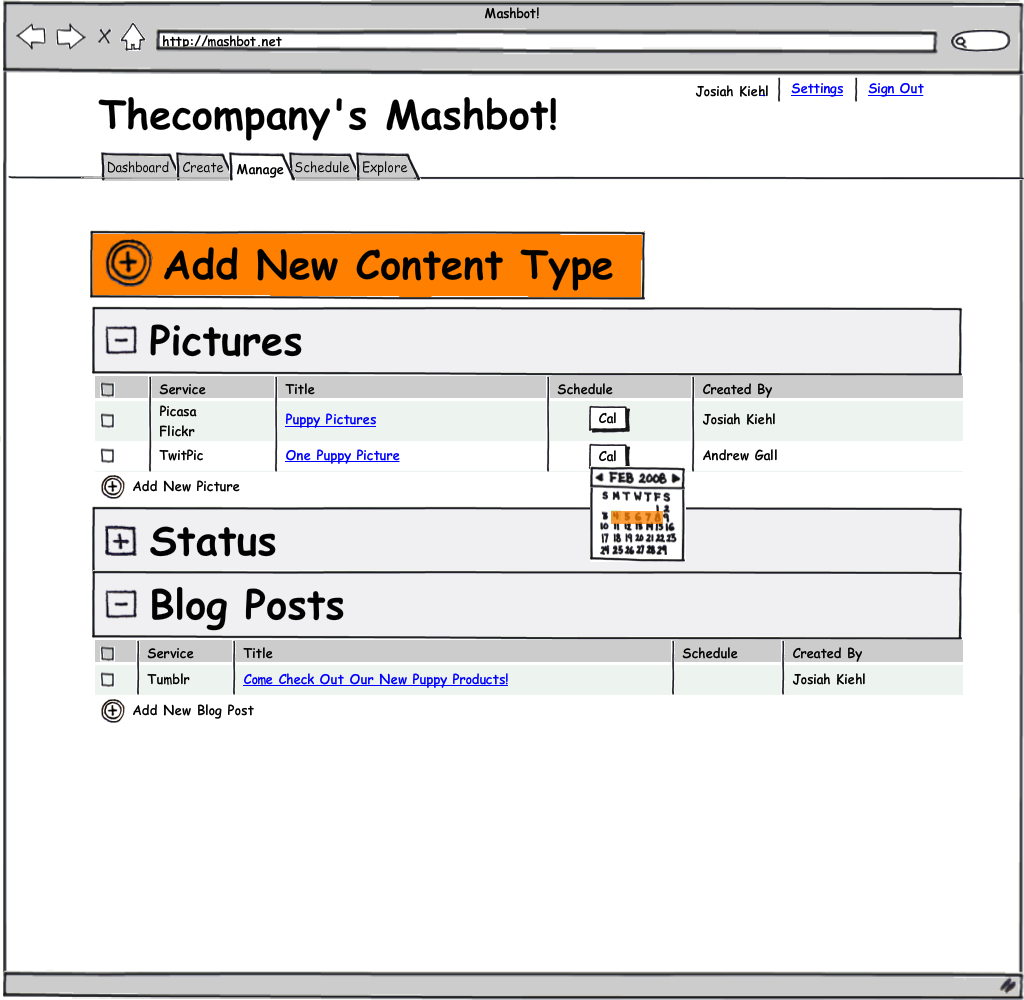
\includegraphics[width=\textwidth]{../mockups/manage-addcontent.png}
		
		}
		\frame{
			\frametitle{}
		
                  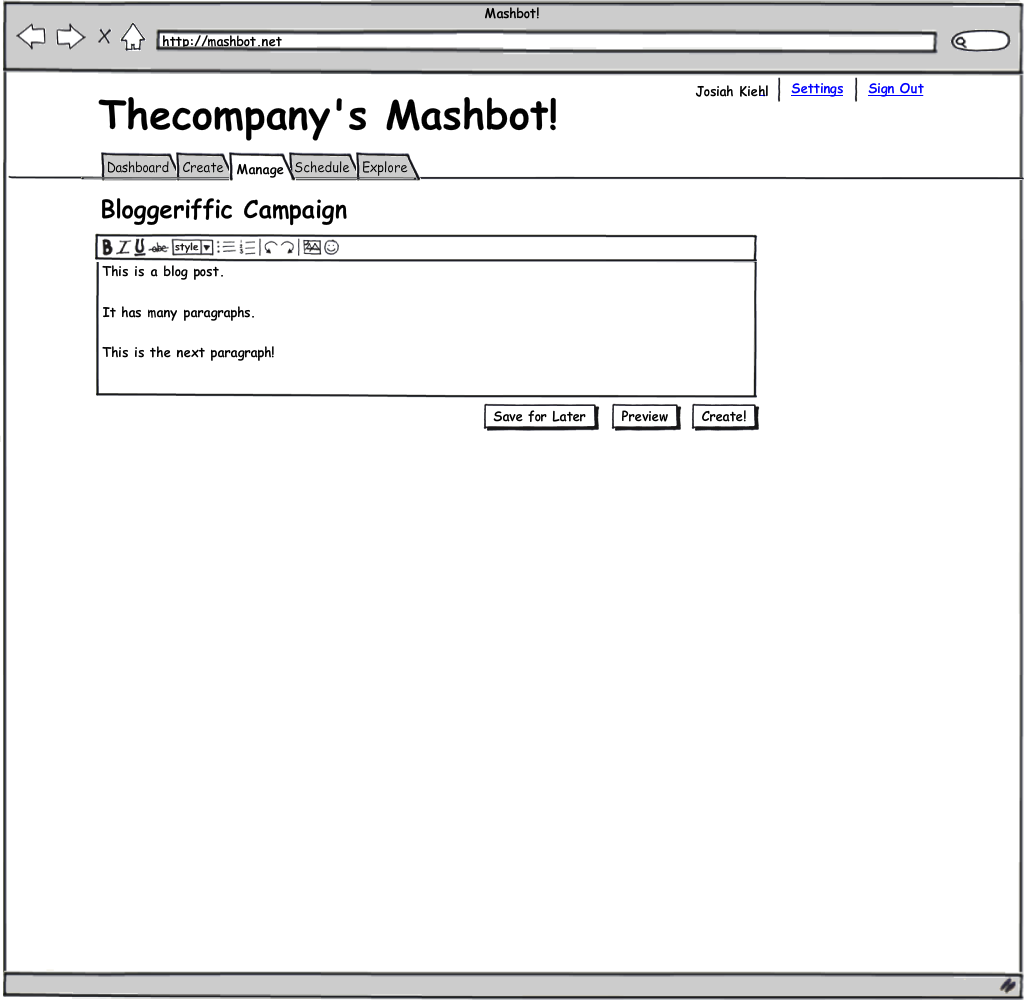
\includegraphics[width=\textwidth]{../mockups/manage-create-blog-post.png}
		
		}
		\frame{
			\frametitle{}
		
                  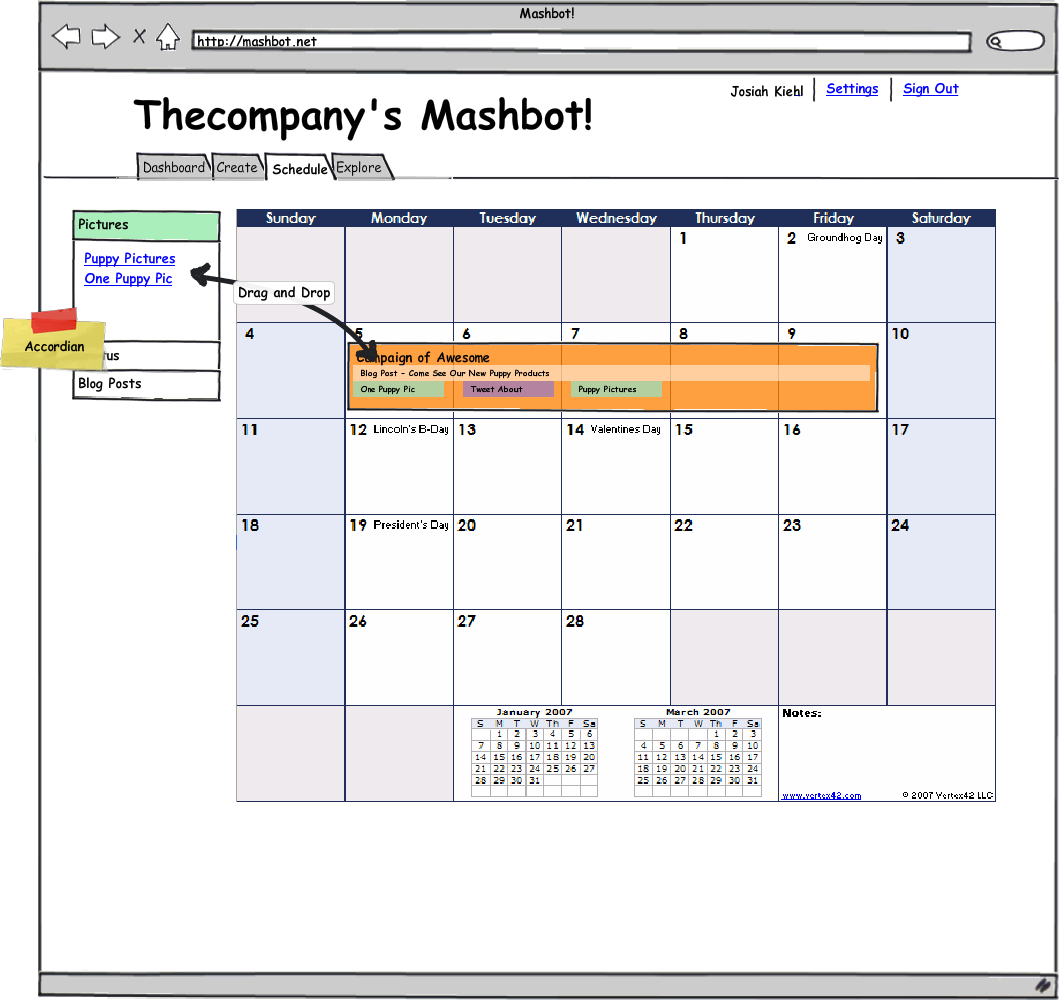
\includegraphics[width=\textwidth]{../mockups/schedule.png}
		
		}
		\frame{
			\frametitle{}
		
                  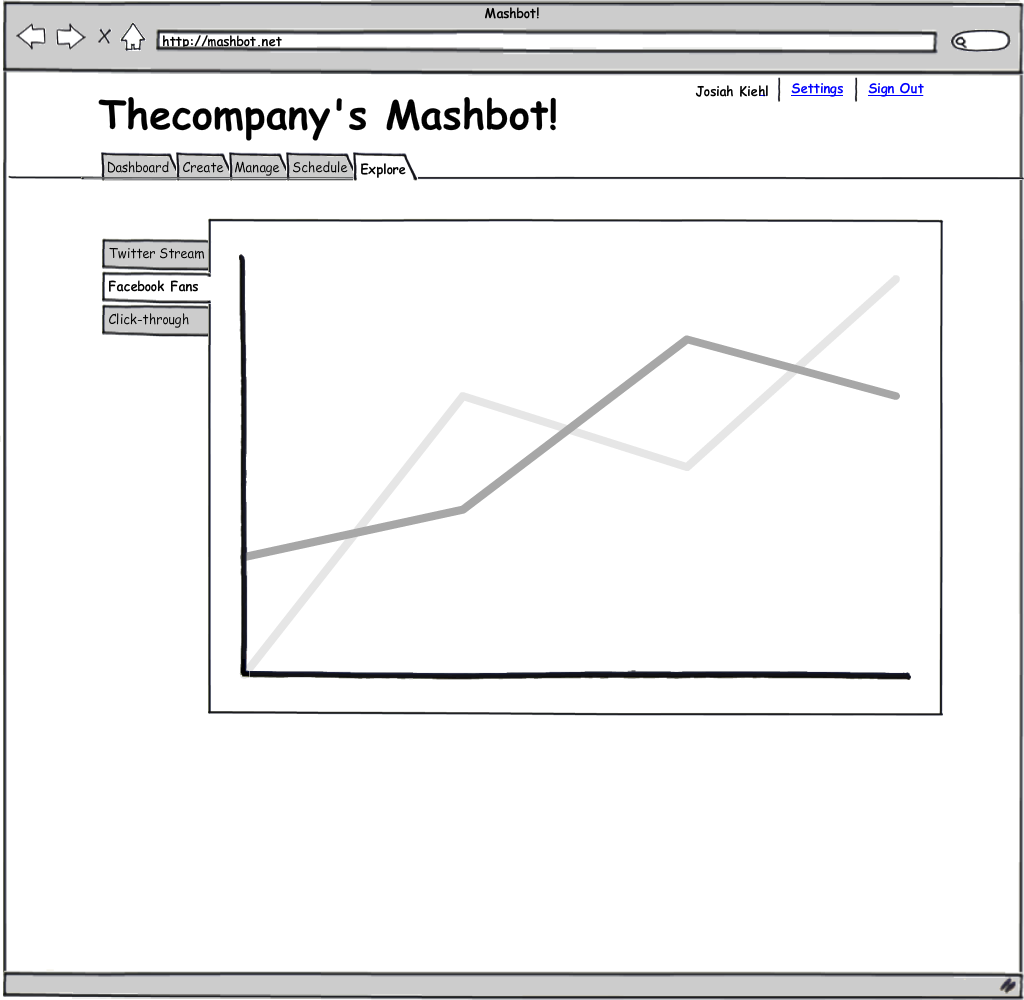
\includegraphics[width=\textwidth]{../mockups/explore-facebook.png}
		
		}
	

\end{document}
